\chapter{Metodologia / Materiais e Métodos}\label{cap:ferramentas}
Esse capítulo abordará em uma sessão o problema proposto por esse trabalho, e logo em seguida, será apresentado um modelo de resolução. O objetivo ao final deste capítulo é poder resolucionar o problema, exibindo seus passos, e atribuir a qualquer outro pesquisador todo o conhecimento necessário para replicar este trabalho através das informações produzidas aqui.

\section{Considerações do Problema}\label{cap:ferramentas:sec:considproblema}

A abordagem do problema referente a essa proposta de mestrado segue uma linha já pequisada por \cite{Lopes}, que seria o \textbf{Problema de Rotulação}. Esse conceito, rotulação de dados,  já é estudado na literatura na área de aprendizagem não-supervisionada, sessão \ref{ssec:aprendNSup}, onde é comum os algoritmos lidarem com os agrupamentos dos dados, e a criação de clusters a partir dos graus de  similaridade entre os elementos.

Muitas pesquisas realizadas na área de rotulação fazem referencia, de fato, a classificação do dados, e não da rotulação, nos termos desse trabalho. Ao agrupar um conjunto de elementos por um derterminado critério, esta havendo uma classificação desses elementos escolhidos, mas pouco se sabe, qual é a compreensão desses grupos, já classificados. 

Existe uma importância na criação dos clusters, contudo para o espectador é interessante existir um rótulo, desse grupo formado, oferecendo elementos em alguma tomada de decisão em razão de seu significado(rótulo).

Tem-se então o real problema de rotulação, contudo é necessário existir algum elemento definindo o porquê daquele grupo formado. O elemento é um rótulo composto por um, ou vários, atributo(s) de maior relevância no cluster, junto com uma faixa de valores. Essa faixa é um intervalo de valores definido pela discretização \ref{cap:refTeor:sec:discret}, onde o intervalo escolhido, seria a faixa que apresenta os valores que se repetem com a maior frequência.

O Problema de Rotulação é formalmente definido como segue abaixo:
\newtheorem{defprob}{Definição}
    \begin{defprob}
    Dado um conjunto de clusters ${C=\{c_1,...,c_k | K \geqslant 1\} }$, de modo que cada cluster contém um conjunto de elementos ${c_i=\{\vec{e}_1,..,\vec{e}_{n^{(c_i)}}|n^{(c_i)} \geqslant 1 \}}$ que podem ser representados por um vetor de atributos definidos em ${\mathbb{R}^m }$ e expresso por ${ \vec{e}^{c_i}=(a_1,..,a_m)  }$ e ainda que  com ${ c_i \cap c_{i'}=\{0\} }$ com ${ 1 \leqslant i, i \leqslant K  }$ e ${ i \neq i' }$.
        \footnotemark 
        \footnotetext{Adaptada de \cite{Lopes}}
        \begin{itemize}[noitemsep]
            \item ${K}$ é o número de clusters;
            \item ${c_i}$ é o i-ésimo cluster qualquer;
            \item ${n^{c_i}}$ é o número de elementos do cluster ${c_i}$;
            \item ${\vec{e}_{n^{(c_i)}}}$ se refere ao j-ésimo elemento pertencente ao cluster ${c_i}$;
            \item ${m}$ é a dimensão do problema;
        \end{itemize}
    \label{teo:problema}
    \end{defprob}

%\afterpage{
%    \begin{quotation}

%        \textit{ Dado um conjunto de clusters ${C=\{c_1,...,c_k | K \geqslant 1\} }$, de modo que cada cluster contém um conjunto de elementos ${c_i=\{\vec{e}_1,..,\vec{e}_{n^{(c_i)}}|n^{(c_i)} \geqslant 1 \}}$ que podem ser representados por um vetor de atributos definidos em ${\mathbb{R}^m }$ e expresso por ${ \vec{e}^{c_i}=(a_1,..,a_m)  }$ e ainda que  com ${ c_i \cap c_{i'}=\{0\} }$ com ${ 1 \leqslant i, i \leqslant K  }$ e ${ i \neq i' }$.
%        }\footnotemark 

%        \footnotetext{Extraída de \cite{Lopes}}
%        \begin{itemize}[noitemsep]
%            \item ${K}$ é o número de clusters;
%            \item ${c_i}$ é o i-ésimo cluster qualquer;
%            \item ${n^{c_i}}$ é o número de elementos do cluster ${c_i}$;
%            \item ${\vec{e}_{n^{(c_i)}}}$ se refere ao j-ésimo elemento pertencente ao cluster ${c_i}$;
%            \item ${m}$ é a dimensão do problema;
%        \end{itemize}
%    \end{quotation}
    %\footnotetext{Extraída de \cite{Lopes}}
%}

\section{O Modelo de Resolução}\label{cap:ferramentas:sec:modeloresolucao}

Uma vez já conhecido a definição do problema - \textit{Definição ~\ref{teo:problema}} - é possível situar a abrangência abordada aqui nessa pesquisa, pois a intenção do estudo científico desenvolvido aqui é provar a realização de \textbf{rotulação de dados com qualquer algoritmo supervisionado}, utilizando as técnicas abordadas neste texto.

O Modelo aqui proposto consiste em apresentar como saída um conjunto de rótulos, onde cada rótulo específico é dado por um conjunto de pares de valores, atributo e seus respectivos intevalos, gerados a partir das frequências dos valores repetidos neste intervalo. Segue \textit{Definição ~\ref{teo:resolucao}} formalizando a saída do modelo:
    \begin{defprob}
    Dado um conjunto de rótulos ${ R=\{ r_{c1},...,r_{ck} \} }$, no qual cada rótulo específico é dados por um conjunto de pares de valores, tem como saída um vetor com atributo e seu respectivo intervalo, ${ r_{ci}=\{ (a_1,[p_1,q_1]),...,(a_{m^{(c_i)}}, ]p_{m^{(c_i)}},q_{m^{(c_i)}}]) \} }$ capaz de melhor expressar o cluster ${c_i}$.
        \footnotemark 
        \footnotetext{Adaptada de \cite{Lopes}}
        \begin{itemize}[noitemsep]
            \item ${k}$ número de rótulos;
            \item ${R}$ representa o conjunto de rótulos na saída do modelo;
            \item ${a}$ é o atributo
            \item ${c_i}$ é o i-ésimo cluster;
            \item ${r_{c_i}}$ é o rótulo referente ao cluster ${c_i}$;
            \item ${]p_{m^{(c_i)}},q_{m^{(c_i)}}]}$ representa o intervalo de valores do atributo ${a_{m^{(c_i)}} }$, onde ${ p_{m^{(c_i)}} }$  é o limite inferior e ${ q_{m^{(c_i)}} }$ é o limite superior;
            \item ${m}$ é a dimensão do problema;
        \end{itemize}
    \label{teo:resolucao}
    \end{defprob}

Como apresentado na sessão \ref{cap:refTeor:sec:trabcorrel}, o autor foca em rotulação automática de grupos utilizando a estratégia de aprendizagem de máquina supervisionada, e paradigma conexionista, para provar seu trabalho. Mas aqui nessa pesquisa foi aplicado no modelo um acréscimo de ${2 (dois)}$ algoritmos com paradigmas de aprendizado diferente do que já foi utilizado, compondo uma base para afirmar, que a partir dessas amostras pode-se fazer rotulação com qualquer algoritmo supervisionado.


\begin{figure}[h!]
        \centering
        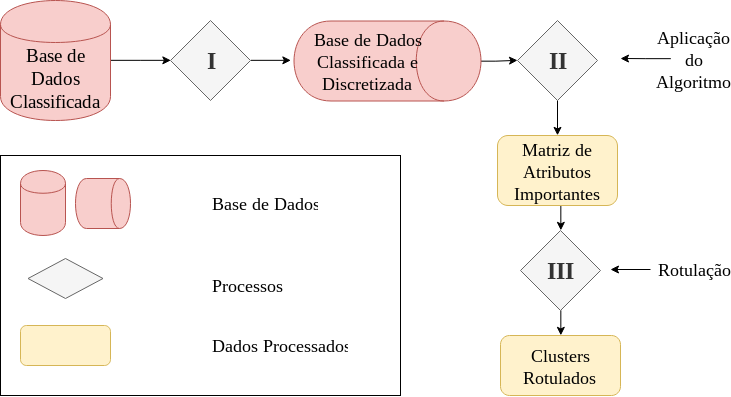
\includegraphics[scale=0.7]{figs/modeloResolucao.png}
        \caption{Modelo de Resolução Proposto} \label{fig:modeloresolucao}
\end{figure}

O modelo, figura \ref{fig:modeloresolucao}, inicialmente mostra a Base de Dados  já classificada, pois o cerne desta pesquisa é conceder ao grupo um significado,a rotulação,  através da técnica de correlação entre atributos, sessão ~\ref{cap:ferramentas:sec:tecnica}. Essa base  conterá  valores contínuos, contudo, conforme modelo será necessário aplicar o método de discretização (I).

Uma vez com a base discretizada ocorre somente a separação dos clusters já classificados de acordo com a própria base de dados\footnote{UCI - Machine Learning Repository. http://archive.ics.uci.edu/ml/ }. Isso é o funcionamento do fluxo (a), que nada mais é do que a separação da base em grupos que já classificados.

No passo (II) é onde serão executados os algoritmos de aprendizagem supervisionado, já visto nas sessões ~\ref{cap:refTeor:sssec:cart} e ~\ref{cap:refTeor:sssec:nbayes}. Essa etapa é umas das mais importantes do método. O algoritmo supervisionado é aplicado várias vezes de acordo com o número de atributos do conjunto de dados, expresso no vetor de tamanho ${m}$. Onde o número de vezes será a quantidade de atributos da base de dados, formando uma tabela contendo valores de zero a cem, de acordo com a importância de cada atributo para o cluster.

Seguindo para o processo (III) acontecerá a escolha do(s) atributo(s) mais relevante(s), selecionado na tabela de atributos importantes, junto com o valor mais frequente desse atributo. Após essa etapa é criado um conjunto de rotulos para cada clusters. O fluxo (b) será utilizado enquanto houver outros algoritmos para serem executados.

\section{Técnica de Correlação entre Atributos }\label{cap:ferramentas:sec:tecnica}

Essa técnica \footnote{Desenvolvida também por \cite{Lopes}} possui um grau de processamento diretamente proporcional a quantidade de características expressa na base de dados definido em ${R^m}$. Ela implica em utilizar todos os atributos, menos o definido como classe, para fazer uma correlação entre eles junto ao algoritmo.


Pegando como exemplo uma base com os seguintes atributos: \textbf{atr1,atr2,atr3,classe}. Exclui o atributo classe, obtêm-se os ${3 (três)}$ primeiros atributos, onde cada um deles será utilizado como classe em refência aos outros atributos. 

Em um primeiro processamento de três, o primeiro atributo \textbf{atr1} se torna classe e executado com os outros dois atributos restantes com um algoritmo supervisionado. O resultado da correlação entre os atributos \textbf{atr2, atr3} em relação ao \textbf{atr1}(figura ~\ref{fig:tecnicamodelo} ) é armazanado em uma matriz, e logo depois é realizado com \textbf{atr2} sendo classe e assim sucessivamente até o último atributo.


\begin{figure}[h!]
        \centering
        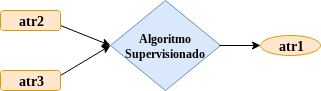
\includegraphics[scale=0.7]{figs/tecnicamodelo.png}
        \caption{Exemplo da técnica aplicada ao atr1 sendo classe } \label{fig:tecnicamodelo}
\end{figure}


\section{Exemplo com Base Modelo Fictícia} \label{cap:ferramentas:sec:exebasemodfic}

Para melhor esclarecer as etapas da figura \ref{fig:modeloresolucao}, a tabela ~\ref{tab:bdm} contém uma base de dados que será utilizada para exemplificar todo o processo do modelo de resolução proposto nesta pesquisa. Logo na primeira coluna da tabela, retém um índice da linha da tabela responsável por identificar cada registro. Os outros campos são atributos que definem características do registro identificado pelo índice da primeira coluna.

\begin{table}[!ht]
\centering
\caption{Base de Dados Modelo}
\label{tab:bdm}
\begin{tabular}{|lllll|}
\hline 
  & atr1 & atr2 & atr3 & classe \\ \hline
1 & 2.08 & 92.11 & 22.07 & 2 \\ \hline
2 & 1.26 & 85.03 & 20.45 & 1 \\ \hline
3 & 2.00 & 108.36 & 22.68 & 2 \\ \hline
4 & 1.74 & 43.78 & 18.72 & 3 \\ \hline
5 & 1.82 & 100.20 & 23.09 & 2 \\ \hline
6 & 1.43 & 77.59 & 21.80 & 1 \\ \hline
7 & 1.53 & 44.01 & 20.98 & 3 \\ \hline
8 & 1.14 & 107.77 & 18.99 & 2 \\ \hline
9 & 1.97 & 98.00 & 22.32 & 2 \\ \hline
10 & 1.50 & 39.67 & 21.78 & 3 \\ \hline
11 & 1.74 & 55.86 & 20.31 & 3 \\ \hline
12 & 1.80 & 65.72 & 19.62 & 1 \\ \hline
13 & 1.33 & 82.01 & 19.82 & 1 \\ \hline
14 & 1.66 & 103.93 & 21.10 & 2 \\ \hline
15 & 1.42 & 66.14 & 21.61 & 1 \\ \hline
16 & 1.87 & 88.36 & 22.45 & 2 \\ \hline
17 & 1.11 & 107.82 & 19.32 & 2 \\ \hline
18 & 2.08 & 67.66 & 20.74 & 1 \\ \hline
19 & 1.85 & 82.65 & 20.35 & 1 \\ \hline
20 & 1.04 & 102.62 & 19.46 & 2 \\ \hline
21 & 1.97 & 100.37 & 21.94 & 2 \\ \hline
22 & 1.95 & 45.70 & 22.10 & 3 \\ \hline
23 & 1.77 & 50.04 & 20.16 & 3 \\ \hline
24 & 1.97 & 81.57 & 19.83 & 1 \\ \hline
25 & 1.52 & 93.13 & 20.61 & 2 \\ \hline
  \end{tabular}
  \begin{tabular}{ |lllll| }
   
\hline
  & atr1 & atr2 & atr3 & classe \\ \hline
26 & 1.42 & 53.51 & 19.64 & 3 \\ \hline
27 & 1.12 & 62.71 & 19.07 & 1 \\ \hline
28 & 2.09 & 60.58 & 20.20 & 1 \\ \hline
29 & 1.95 & 69.23 & 19.68 & 1 \\ \hline
30 & 1.03 & 47.81 & 19.47 & 3 \\ \hline
31 & 1.75 & 90.92 & 21.39 & 2 \\ \hline
32 & 1.72 & 42.35 & 22.89 & 3 \\ \hline
33 & 1.47 & 101.77 & 19.20 & 2 \\ \hline
34 & 1.53 & 41.16 & 22.67 & 3 \\ \hline
35 & 1.44 & 93.61 & 21.03 & 2 \\ \hline
36 & 1.51 & 98.65 & 19.24 & 2 \\ \hline
37 & 1.06 & 68.82 & 21.68 & 1 \\ \hline
38 & 1.48 & 80.40 & 21.43 & 1 \\ \hline
39 & 1.14 & 61.59 & 19.90 & 1 \\ \hline
40 & 1.08 & 91.93 & 20.81 & 2 \\ \hline
41 & 1.62 & 79.21 & 18.43 & 1 \\ \hline
42 & 1.68 & 80.87 & 18.42 & 1 \\ \hline
43 & 1.81 & 98.24 & 22.13 & 2 \\ \hline
44 & 1.30 & 69.27 & 18.83 & 1 \\ \hline
45 & 1.80 & 101.21 & 21.61 & 2 \\ \hline
46 & 1.79 & 72.02 & 22.02 & 1 \\ \hline
47 & 1.56 & 81.71 & 22.10 & 1 \\ \hline
48 & 1.98 & 77.16 & 21.71 & 1 \\ \hline
49 & 1.86 & 89.12 & 22.84 & 2 \\ \hline
50 & 1.55 & 76.01 & 19.74 & 1 \\ \hline
\end{tabular}
\end{table}

Seguindo a definição ~\ref{teo:problema} um elemento é expresso por um vetor  de dimensão ${m}$, com tamanho igual ao número de atributos. Um exemplo do elemento 2 da tabela ~\ref{tab:bdm}, pode ser representado por ${\vec{e}_{2}=(1.26,85.03, 20.45)}$.

\subsection{Processo (I) - Discretização} \label{cap:ferramentas:ssec:disc}

Segundo \cite{Catlett2006, Hwang2002} o processo de discretização na etapa de treinamento pode aumentar a acurácia do algoritmo de aprendizado supervisionado. Dessa maneira a etapa de discretização ganha um papel importante no modelo, e também no processo de Rotulação (III), pois é utilizada uma inferência na faixa discretizada para encontrar o intervalo na faixa.

Para esse exemplo será utilizada a técnica de discretização por frequências iguais - EFD - e divisão de números de faixas igual a R=3. Na figura\footnote{Figura adaptada de \cite{Lopes}} \ref{fig:EFD_R_3} poderá ser vizualizado como é feita a discretização.
 \begin{figure}[h!]
    \centering
    \subfloat[Discretização em atr1]{
        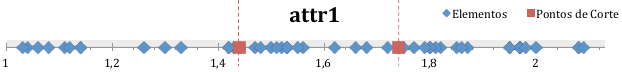
\includegraphics[scale=0.8]{figs/discretizacaoEFD_R_3_atr1.png}
        \label{fig:EFD_R_3:efd:atr1} }
    
    \subfloat[Discretização em atr2]{
        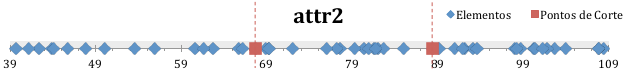
\includegraphics[scale=0.8]{figs/discretizacaoEFD_R_3_atr2.png}
        \label{fig:EFD_R_3:efd:atr2} }
    
    \subfloat[Discretização em atr3]{
        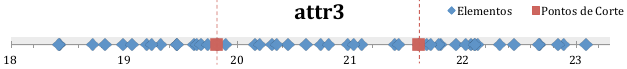
\includegraphics[scale=0.8]{figs/discretizacaoEFD_R_3_atr3.png}
        \label{fig:EFD_R_3:efd:atr2} } 
    
    \caption{Discretização de atributos utilizando EFD com R = 3} \label{fig:EFD_R_3}
        
        %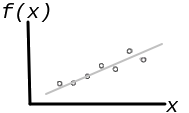
\includegraphics[scale=0.4]{figs/grafB.png}
        %\caption{Polinômio Superajustado} \label{grafB}
\end{figure}
Através da figura \ref{fig:EFD_R_3} fica claro o conteúdo da faixa 1, contendo os valores iniciais até o primeiro ponto de corte, na faixa 2, são os valores após o primeiro ponto de corte até o segundo ponto de corte. E na faixa 3 contém todos  valores a partir do segundo ponto de corte.


\begin{table}[!ht]
\centering
\caption{Base de Dados Modelo Discretizada}
\label{tab:bdmd}
\begin{tabular}{|lllll|}
\hline 
  & atr1 & atr2 & atr3 & classe \\ \hline
1	&	3	&	3	&	3	&	2	\\	\hline
2	&	1	&	2	&	2	&	1	\\	\hline
3	&	3	&	3	&	3	&	2	\\	\hline
4	&	2	&	1	&	1	&	3	\\	\hline
5	&	3	&	3	&	3	&	2	\\	\hline
6	&	1	&	2	&	3	&	1	\\	\hline
7	&	2	&	1	&	2	&	3	\\	\hline
8	&	1	&	3	&	1	&	2	\\	\hline
9	&	3	&	3	&	3	&	2	\\	\hline
10	&	2	&	1	&	3	&	3	\\	\hline
11	&	2	&	1	&	2	&	3	\\	\hline
12	&	3	&	1	&	1	&	1	\\	\hline
13	&	1	&	2	&	1	&	1	\\	\hline
14	&	2	&	3	&	2	&	2	\\	\hline
15	&	1	&	1	&	2	&	1	\\	\hline
16	&	3	&	2	&	3	&	2	\\	\hline
17	&	1	&	3	&	1	&	2	\\	\hline
18	&	3	&	1	&	2	&	1	\\	\hline
19	&	3	&	2	&	2	&	1	\\	\hline
20	&	1	&	3	&	1	&	2	\\	\hline
21	&	3	&	3	&	3	&	2	\\	\hline
22	&	3	&	1	&	3	&	3	\\	\hline
23	&	3	&	1	&	2	&	3	\\	\hline
24	&	3	&	2	&	2	&	1	\\	\hline
25	&	2	&	3	&	2	&	2	\\	\hline
  \end{tabular}
  \begin{tabular}{ |lllll| }
   
\hline
  & atr1 & atr2 & atr3 & classe \\ \hline
26	&	1	&	1	&	1	&	3	\\	\hline
27	&	1	&	1	&	1	&	1	\\	\hline
28	&	3	&	1	&	2	&	1	\\	\hline
29	&	3	&	2	&	1	&	1	\\	\hline
30	&	1	&	1	&	1	&	3	\\	\hline
31	&	3	&	3	&	2	&	2	\\	\hline
32	&	2	&	1	&	3	&	3	\\	\hline
33	&	2	&	3	&	1	&	2	\\	\hline
34	&	2	&	1	&	3	&	3	\\	\hline
35	&	1	&	3	&	2	&	2	\\	\hline
36	&	2	&	3	&	1	&	2	\\	\hline
37	&	1	&	2	&	3	&	1	\\	\hline
38	&	2	&	2	&	2	&	1	\\	\hline
39	&	1	&	1	&	2	&	1	\\	\hline
40	&	1	&	3	&	2	&	2	\\	\hline
41	&	2	&	2	&	1	&	1	\\	\hline
42	&	2	&	2	&	1	&	1	\\	\hline
43	&	3	&	3	&	3	&	2	\\	\hline
44	&	1	&	2	&	1	&	1	\\	\hline
45	&	3	&	3	&	2	&	2	\\	\hline
46	&	3	&	2	&	3	&	1	\\	\hline
47	&	2	&	2	&	3	&	1	\\	\hline
48	&	3	&	2	&	3	&	1	\\	\hline
49	&	3	&	3	&	3	&	2	\\	\hline
50	&	2	&	2	&	1	&	1	\\	\hline

\end{tabular}
\end{table}

A tabela \ref{tab:bdmd} é o resultado após a discretização de todos os atributos. Contudo sabe-se que ao se lidar com valores discretos onde cada intervalo representa uma faixa de valores poderá o algoritmo está perdendo um pouco de informação, mas por outro lado essa decisão tornará o aprendizado mais fácil de interpretar e com respostas mais rápidas.

\subsection{Processo (II) - Algoritmos Supervisionados}\label{cap:ferramentas:ssec:algsuper}

Ao chegar nessa etapa, Processo (II) da figura \ref{fig:modeloresolucao}, já se tem uma base discretizada e clusters formados, tabela \ref{tab:bdmd}. Agora é feita a execução do algorimo de aprendizado supervisionado e identificado os atributos de maior importância de cada cluster.

Uma vez com o conhecimento do cluster, serão percorridos todos os atributos, onde a cada iteração um atributo será a classe da vez. Nesse exemplo primeiramente o atributo \textbf{atr1} será classe, e os demais irão participar como entrada junto ao algoritmo, e verificar seu grau de importância entre eles. Depois o atributo \textbf{atr2} irá ser classe, e depois o \textbf{atr3}, fechando o ciclo de todos os atributos do cluster. Como visualizado na figura \ref{fig:tecnicamodelocomp} 
\begin{figure}[h!]
        \centering
        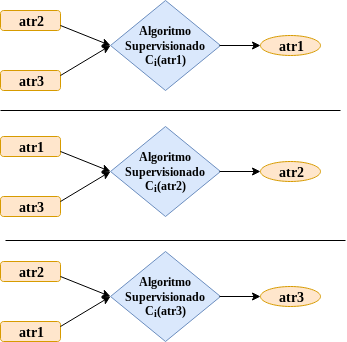
\includegraphics[scale=0.7]{figs/tecnicamodeloComp.png}
        \caption{Exemplo da técnica aplicada aos ${3 (três)}$ atributos, cada um sendo classe em determinada iteração } \label{fig:tecnicamodelocomp}
\end{figure}

Essa correlação entre os atributos junto com a aplicação dos algoritmos geram uma matriz de atributos importantes. O quão relevante o atributo será em relação ao cluster ${c_i(atr)}$, será dado em uma porcentagem de acerto quando aplicado como saída na execução de um algorimo supervisionado. Quanto maior sua porcentagem, mais correlacionado é o atributo em relação ao demais(figura \ref{fig:rotulacao}), logo ele é considerado um atributo bem relevante. Sendo assim esse atributo poderá resumir as características do problema, podendo ser considerado atributo mais importante e escolhido como rótulo.

 \begin{figure}[h!]
    \centering
    \subfloat[Execução do Naive Bayes]{
        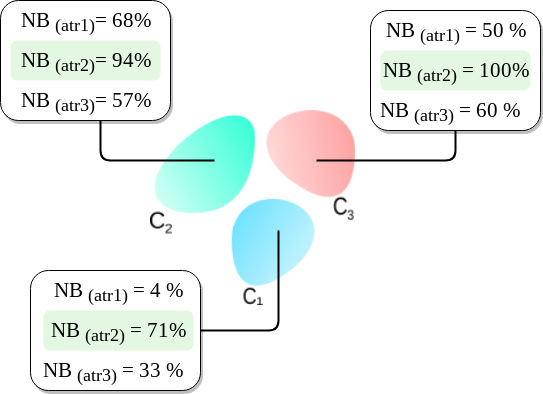
\includegraphics[scale=0.3]{figs/rotulacaoNB.png}
        \label{fig:rotulacao:rotNB} }
    \quad
    \subfloat[Execução do algorimo de Árvore de Decisão]{
        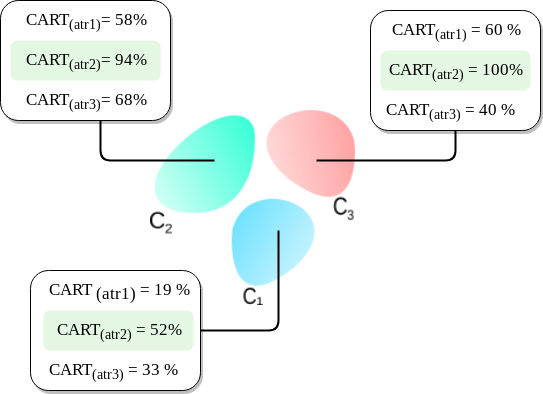
\includegraphics[scale=0.3]{figs/rotulacaoDecisionTree.png}
        \label{fig:rotulacao:rotDT} } 
    
    \caption{Resultado dos Algoritmos} \label{fig:rotulacao}
        %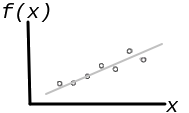
\includegraphics[scale=0.4]{figs/grafB.png}
        %\caption{Polinômio Superajustado} \label{grafB}
\end{figure}

Na figura \ref{fig:rotulacao:rotNB} mostra o resultado da execução do Naive Bayes em cima da Base Modelo e exibe os resultados em porcentagem de acerto de cada atributo em relação aos demais. O mesmo acontece com a figura \ref{fig:rotulacao:rotDT} onde é aplicado um algorimo de Árvore de Decisão, exibindo o resultado de todas as taxas de acerto, em porcentagem, dos atributos de seus respectivos clusters.

Uma forma de eliminar uma possível ambiguidade entre os clusters foi adicionar uma variável  ${V}$. Com essa variável a seleção dos atributos rótulos de um clusters, seram todos os atributos que tiverem até uma diferença ${V}$ em relação ao atributo de maior taxa de acerto, expresso em porcentagem. Portanto se o atributo de maior taxa de acerto possuir ${90\%}$, e o ${V=10\%}$  então todos outros atributos que tiverem valores a partir de ${80\%}$ seram selecionados como rótulo do cluster.  

O valor da variável ${V}$ é subjetivo e irá ser arbitrado de acordo com os resultados em cada aplicação do algoritmo em cima de um conjunto de dados. Nese exemplo os atributos importantes com ${V=12}$ utilizando a figura \ref{fig:rotulacao:rotNB}, teriam os rótulos,por clusters, ${r_{c_i}}$ : ${r_{c_1}=\{atr2\}}$, ${r_{c_2}=\{atr2\}}$, ${r_{c_3}=\{atr2\}}$.

\subsection{Processo (III) - Rotulação}

Nesse processo de rotulação serão calculados os intervalos dos atributos que estão na figura \ref{fig:modeloresolucao} como Atributos Importantes, selecionados na etapa anterior. Para compor o rótulo ${r_{c_i}}$ do cluster ${c_i}$ é calculado a faixa do atributo  que tiver maior frequência. 
É possível verificar neste exemplo, da Base Modelo, o resultado da figura \ref{fig:rotulacao:rotNB}, onde o rótulo ${r_{c_1}}$ é o  \textbf{atr2=]67.66, 88.36]}, porque o valor da faixa de maior frequência do cluster ${c_1}$ em relação ao atributo \textbf{atr2} é a faixa 2(figura \ref{fig:EFD_R_3:efd:atr2}), que é representa o limite inferior ${]67.66}$s e o limite superior, ${88.36]}$.

Uma vez terminado o processo (III) de rotulação, o fluxo ${b}$ da figura \ref{fig:modeloresolucao}, só será seguido, caso seja necessário para execução de outro algoritmo.

Contudo pode-se definir os rótulos nesta etapa da seguinte maneira:


\begin{itemize}[noitemsep]
            \item Algoritmo Naive Bayes  \ref{fig:rotulacao:rotNB} aplicado na BD Modelo
            \subitem ${r_{c_1}=(atr2,]67.66, 88.36])}$;
            \subitem ${r_{c_2}=(atr2,]88.36, 108.36])}$ ;
            \subitem ${r_{c_3}=(atr2,[39.67, 67.66])}$;
            
            \item Algoritmo de Árvore de Decisão  \ref{fig:rotulacao:rotDT} aplicado na BD Modelo
            \subitem ${r_{c_1}=(atr2,]67.66, 88.36])}$;
            \subitem ${r_{c_2}=(atr2,]88.36, 108.36])}$ ;
            \subitem ${r_{c_3}=(atr2,[39.67, 67.66])}$;
\end{itemize}

Logo abaixo o algoritmo \ref{alg:rotulacao} exibe a rotina em forma de pseudocódigo para melhor entendimento.

\IncMargin{1em}
\begin{algorithm}[h]

\nl $Carrega\_valores\_auxiliares(V,R,TipoDiscretização)$\;
\nl $Carrega\_BD$\; 
\nl $Discretiza\_BD$\; 
\nl $Separa\_em\_clusters\_de\_acordo\_com\_classificação\_BD$\; 
\nl \While{existir clusters}{
 \nl \While{existir atributos}{ 
      \nl $prepara\_vetor\_atributos/classe$\; 
      \nl $Aplica\_algoritmo\_supervisionado$\;
      \nl $Calcula\_matriz\_de\_porcentagem\_de\_acertos$\; 
      } 
    \nl $Carrega\_atributos\_importantes\_considerando\_V$\;
    \nl $Associa\_valores\_aos\_intervalos$\; 
 }
 \nl $Exibe\_rótulos\_todos\_clusters$\; 
 \caption{Rotina de Rotulação}\label{alg:rotulacao}
 
\end{algorithm}
\DecMargin{1em}
        
